\documentclass[14pt,fleqn]{article}
\usepackage{mathrsfs}
\usepackage{latexsym,amsmath,amssymb}
\usepackage{bbm}
\usepackage{amsfonts}
\usepackage{caption}
\usepackage{mathrsfs}
\usepackage{amsfonts}
\usepackage{color}
\usepackage{graphicx}
\usepackage{epstopdf}
\usepackage{amssymb}
\usepackage{amsthm}
\usepackage{amsmath}
\usepackage{bbm}
\usepackage{booktabs}
\usepackage{makecell}
\usepackage{float}
\newtheorem{Lem}{Lemma}{}
\usepackage{pifont}
\usepackage{color,xcolor}
\usepackage{stmaryrd}
\usepackage{bbding}
\usepackage{mathrsfs}
\setlength{\parskip}{-1.5ex}
\pagenumbering{arabic}
\renewcommand{\baselinestretch}{1.2}
\usepackage{latexsym}
\usepackage{graphicx}
\usepackage{amsmath}
\usepackage{amssymb}
\usepackage{tabularx}
\usepackage{multirow}
\usepackage{adjustbox}
\usepackage{array, caption, threeparttable}
\usepackage[font=small,labelfont=bf,labelsep=none]{caption}
%表格编号Table 1 可以加粗显示
\captionsetup[table]{
	labelfont = bf,    % "Table X" 加粗
	%textfont = it,     % 标题文本斜体（根据期刊要求调整）
	%labelsep=newline,%换行
	justification = centering,
	singlelinecheck = false, % 允许换行
	labelsep = period,  % 编号和标题间空格sapce,period加点,不加space、period这两个就是冒号
	skip = 6pt         % 标题与表格间距
}
\textheight=22cm\textwidth=15.6cm \oddsidemargin=0.25in
\evensidemargin=0.25in
\date{}
\renewcommand\baselinestretch{1.0}
 \linespread{1.15}
\begin{document}
\captionsetup[figure]{labelfont={bf},labelformat={default},labelsep=period,name={Fig.}}

\title{\bf Response Letter for 9418778}
\author{}
\date{}
\maketitle
\noindent \textbf{Paper ID:} 9418778 \\
\textbf{Paper title:} Adaptive Event-Triggered Control for Interval Type-2 Fuzzy Cyber-Physical Systems Under Deception Attacks and Actuator Failures: A Membership-Function-Derivative-Dependent Switching Perspective\\
\textbf{Authors:} Xiaoqing Li, Haoxiang Zhao, Yu Yang, Jun Cheng, Kaibo Shi \\
\textbf{Corresponding author:} Yu Yang
\\
\\
\\
\noindent \textbf{Dear Editors and Reviewers}: \\
\indent Thank you for your letter and for the editors’ and reviewers’ valuable comments on our manuscript entitled
“Adaptive Event-Triggered Control for Interval Type-2 Fuzzy Cyber-Physical Systems Under Deception Attacks and Actuator Failures: A Membership-Function-Derivative-Dependent Switching Perspective” (9418778). We appreciate the constructive feedback, which is very helpful for improving our paper. We have carefully considered all comments and made corresponding revisions. The main changes and our responses are summarized as follows:
\\
~\\
\\
\textbf{Response to  Editor in Chief:}\\[10pt]
*****************************************************************************************\\
\\
\hspace*{-0.5cm}\indent\textbf{Reviewer $\sharp$ 1:} This manuscript investigates adaptive event-triggered control for interval type-2 (IT-2) fuzzy cyber-physical systems subject to stochastic deception attacks and Markov-type actuator failures. The combination of adaptive transmission and membership-function-derivative-dependent regional control is relevant to secure networked control. The numerical examples provide an initial illustration of the proposed framework. After reading, the primary features and contributions of this article are sound compared to some existing publications. However, the following aspects should be seriously considered to improve the presentation quality of this investigation.
\\
~\\
\textbf{1.} It is noted that your manuscript needs careful editing, such as the English grammar and sentence structure so that the goals and results in your work are friendly to the weak in English.
\\[10pt]
\indent \textbf{Reply 1:}We sincerely appreciate your constructive suggestions. The following provides our detailed clarifications and corresponding revisions point by point. \\


1) The outliers discussed in this paper refer to deviations in the numerical values of the measurement output $y(t,\eth)$. In this study, attacks, disturbances, and faults are regarded as factors that may cause abnormal variations in the measured output $y(t,\eth)$, and these factors are collectively referred to as abnormal disturbance. When the measurement or transmission process of $y(t,\eth)$ is affected by such abnormal disturbance, the measured output exhibits a certain deviation relative to the true value of $y(t,\eth)$. Evidently, these data are outliers and cannot accurately reflect the true state information of the neural network being estimated.\\

The relevant concepts have been thoroughly refined and clarified in the revised manuscript as follows:\\

``Measurement outliers refer to data points that significantly deviate from the overall data trend, {\color{red}primarily caused by abnormal disturbances. Typical sources of such abnormal disturbances include sensor faults, network attacks, and environmental variations. These abnormal disturbances lead to large measurement deviations between the measured and actual values, resulting in outliers that degrade estimation accuracy and may even severely impair RSE."}(The fourth paragraph in the introduction)\\

2) An outlier represents a numerical abnormality in the output $y(t,\eth)$, which remains an inherent characteristic of $y(t,\eth)$ itself. Similar to the existing studies on outlier-resilient estimation (see https://doi.org/10.1007/s11071-024-09404-2; 10.1109/TNNLS.2020.2991151), this paper characterizes the influence of measurement outliers through variations in the numerical values of $y(t,\eth)$. Consequently, the transmission of such corrupted measurement data to the estimator inevitably affects the estimation accuracy.\\

3) The explanation of the saturation function is provided in Remark 2.4 of this paper, and here we further elaborate on its role in mitigating outliers.
\\

\textbf{Remark 2.4.} To effectively mitigate the influence of such outliers, a saturation function (4) is introduced in the proposed ORSE. The parameter $\kappa_{\text{max}}$ represents the saturation level. The saturation function (4) suppresses outliers by enforcing upper and lower bounds on the measurements. {\color{red}Specifically, when the measurement data are not outliers, the output of the saturation function (4) equals its input, ensuring that the transmitted data accurately reflect the true state of the estimated system. Conversely, when the measurement data are outliers, the output of the saturation function (4) is constrained to its upper or lower bound (depend on the sign of the outlier). Hence, the saturation function (4) effectively suppresses the impact of large outliers by limiting their magnitude, thereby reducing the estimation error.} The value of $\kappa_{\text{max}}$ can be determined a priori based on engineering practice, reflecting the confidence in the measurement output. In this sense, the saturation function (4) is confidence-dependent. Notably, in the absence of the saturation function, ORSE (3) simplifies to a conventional resilient state estimator.\\

4) How does the abnormal disturbance presented in figure 3 is incorporated into the system model? It seems that there are no theoretical derivations associated with it in the modelling part.\\

In this paper, the term abnormal disturbance collectively refers to factors that cause measurement data to deviate and become outliers. In Fig. 3, the horizontal axis represents the occurrence time of the abnormal disturbance, while the vertical axis indicates the measurement deviation induced by the disturbance (i.e., the deviation that transforms normal measurements into outliers). Fig. 3 illustrates the occurrence times and specific values of outliers in Numerical Example 1. For instance, according to Table 1, the measurement data at $t=15$ are identified as outliers, with the corresponding value given by $y(15,\eth)+10$.\\
\begin{figure}[H]
	\centering
	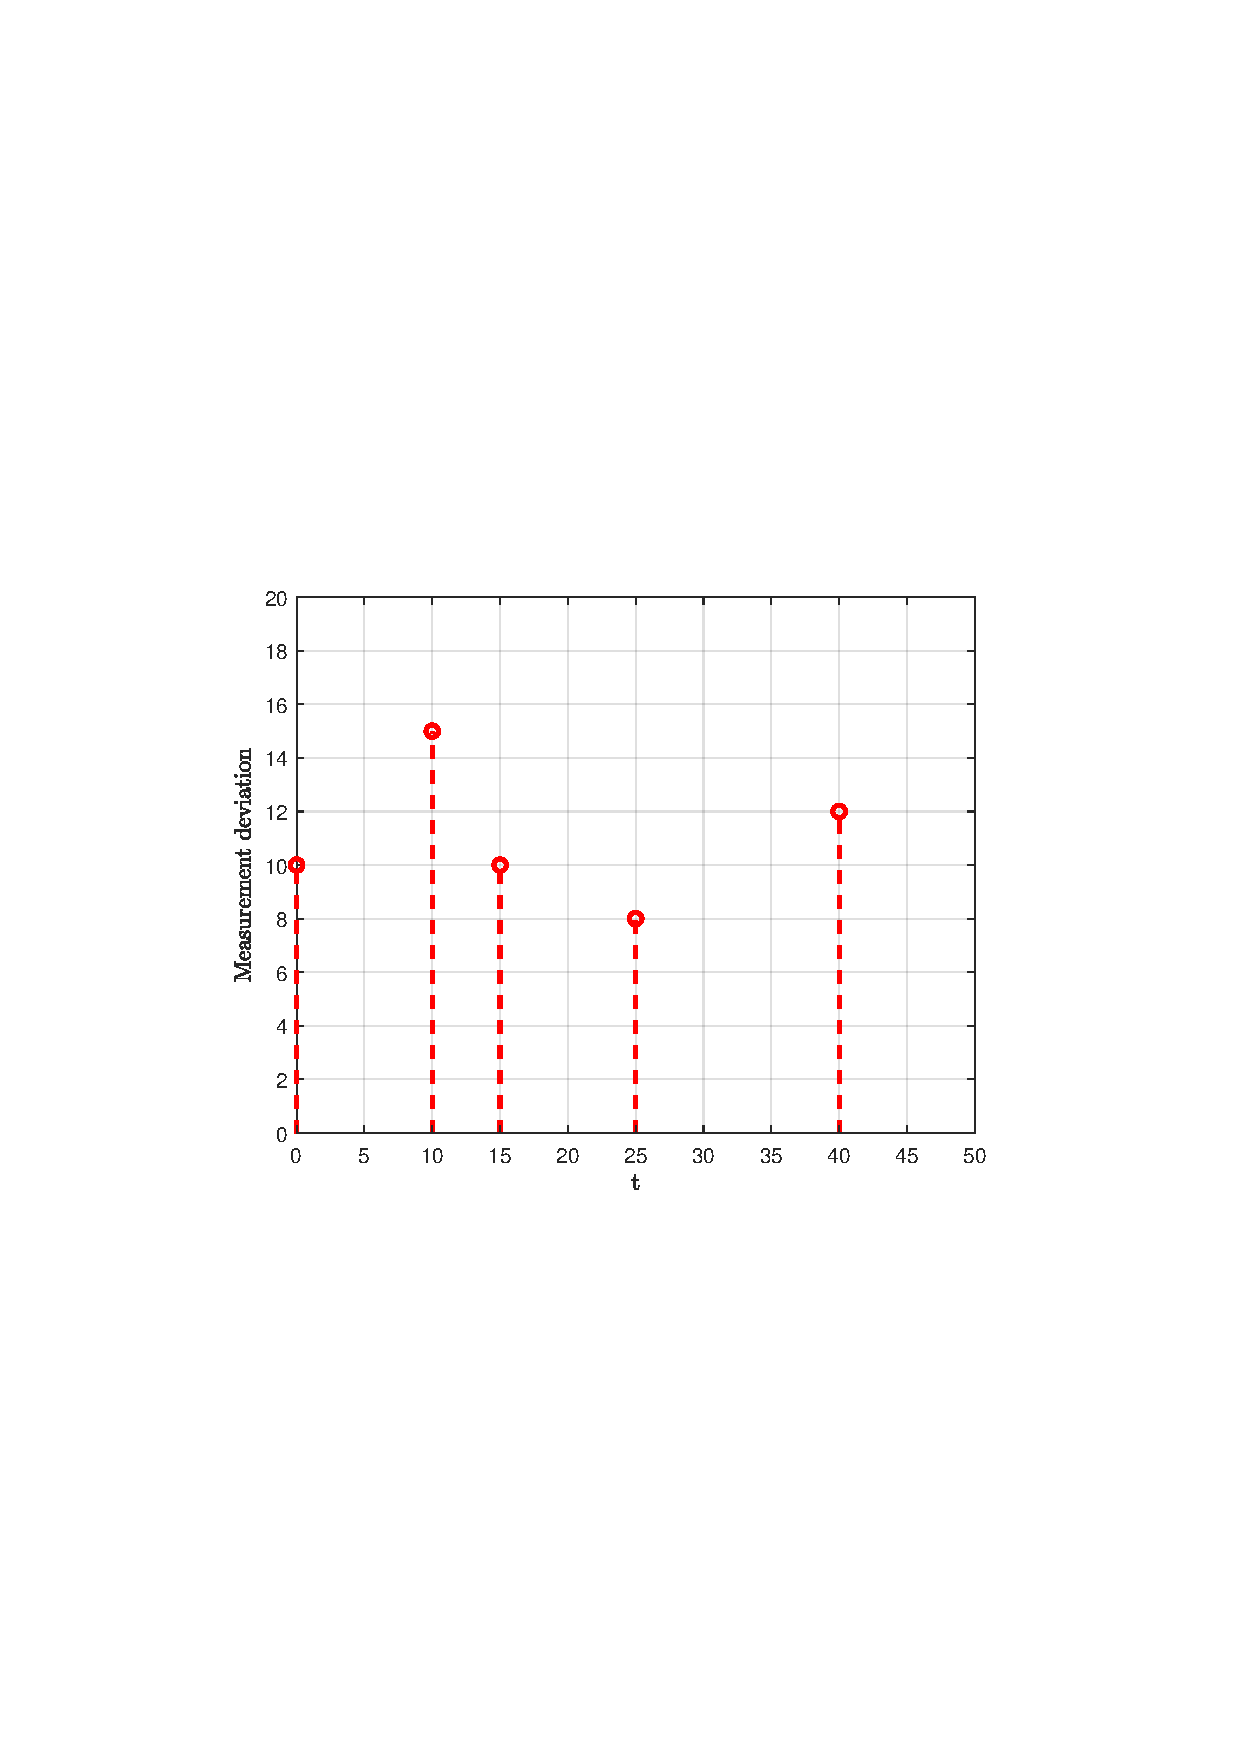
\includegraphics[width=3.5in]{outlier.pdf}
	\caption{\color{red}Measurement deviation caused by abnormal disturbance.}
	\label{Fig.4}
\end{figure}

Thank you once again for your valuable feedback regarding the relevant concepts in this paper. We hope that these revisions will improve the logical structure and coherence of the manuscript, making the connection between key concepts and related work clearer. Your suggestions will undoubtedly help enhance the presentation of the research.

~\\
\\
\textbf{2.} \textcolor{red}{The} motivation for jointly considering deception attacks, actuator failures, and communication limitations needs clarification. Could the authors clarify why these factors require simultaneous consideration and how their combined effects influence closed-loop stability and $\mathrm{H}_{\infty}$ performance?
\\[10pt]
\indent \textbf{Reply 2:} Thank you for this comment.\\

In Eq.~(15), the actuator scales a command based on the most recently released sample. If that sample was falsified, the feedback may continue to use incorrect data while an actuator fault reduces the effectiveness of the command. This can impair the controller's ability both to drive the state back to equilibrium and to attenuate external disturbances. We revised the last two sentences of the following paragraph in the Introduction.\\

\textbf{Introduction (p.~2).} In addition to cyber-layer risks and communication constraints, physical-layer reliability is also critical for CPSs. Actuators may suffer from hardware aging, mechanical wear, or harsh operating environments, which can cause stochastic degradation of the control channel [27, 28]. Markov processes are commonly used to describe switching among different actuator failure modes [29, 30]. If such failures are not considered in controller design, the resulting control input may be weakened or distorted. \textcolor{red}{With event-triggered transmission, the controller may continue to use a falsified sample until the next release, while an actuator fault may weaken the command computed from that sample. These effects must therefore be considered together when assessing whether the feedback can stabilize the plant and achieve the prescribed $\mathrm{H}_\infty$ disturbance attenuation.}

~\\
\\
\textbf{3.} The author should check the References carefully throughout this paper, there are many references which not fit our style need some modification and there is something wrong with the formatting of the Reference.
\\[10pt]
\indent \textbf{Reply 3:} Thanks to you for your good comment. \\

Compared with the traditional LKF, the proposed asymmetric LKF offers two main advantages.\\

First, the matrix $R_2$ in the LKF $V_2(t)$ is not required to be symmetric, and when $R_2=0$, $V_2(t)$ naturally degenerates into the conventional LKF. Second, the proposed asymmetric LKF relaxes the positive definiteness constraint on all associated matrices, thereby reducing conservatism compared with traditional LKF. A detailed explanation of the proposed asymmetric LKF, along with an analysis of its computational complexity, is provided in Remark 3.1.\\

\textbf{Remark 3.1.} It is noteworthy that an important characteristic of $V_1(t, \eth)$ is its dependence on the system mode. In addition, unlike conventional LKFs, the constructed $V_2(t, \eth)$ is asymmetric. However, when $R_2 = 0$ in Theorem 3.1, $V_2(t, \eth)$ degenerates into a symmetric form. Moreover, the positive definiteness condition of this LKF is more relaxed compared to traditional LKF, requiring only the matrices $\Theta_{1}$, $\Theta_{2u}$, $T$ and $N D_k$ to be positive definite, without imposing positive definiteness on all related matrices, thereby reducing the conservatism in the analysis process. {\color{red} Furthermore, for the $u$th semi-Markov mode in Theorem 3.1, the number of decision variables is $n[8.5n+0.5(\mathcal{N}+1)( \mathcal{N}+2)n+(\mathcal{N}+10)n+5.5]$. It is worth noting that if $V_2(t, \eth)$ were replaced by a general symmetric augmented LKF of the form $V_2(t, \eth) = \int_\Omega \int_{t-\wp}^t \left[\vartheta^\text{T}(\nu, \eth), \int_\nu^t \vartheta^\text{T}(\mu, \eth) d\mu \right] R \left[ \vartheta^\text{T}(\nu, \eth), \int_\nu^t \vartheta^\text{T}(\mu, \eth) d\mu \right]^\text{T} d\nu \, d\eth$, where $R \in \mathbb{R}^{2n \times 2n}$ is positive define matrix, the resulting $V_2(t, \eth)$ would significantly increase the complexity of condition (12), thereby raising the computational complexity.}



~\\
\\
\textbf{4.} \textcolor{red}{Please} clarify the physical meaning of the actuator-failure parameters $F_{i0}$, $F_{i1}$ and the Markov transition-rate matrix used in the simulation. How are the failure-level bounds and the transition rates chosen, and does the closed-loop system remain stable under more severe failure modes?
\\[10pt]
\indent \textbf{Reply 4:} Thank you for this comment.\\

1) In Eq.~(13), $F_{i0}$ gives the midpoint of the actuator effectiveness interval in mode $i$, and $F_{i1}$ gives its half-width. We chose two illustrative levels of partial loss for the simulations. The intervals are $[0.8,1.0]$ in mode~1 and $[0.6,1.0]$ in mode~2, corresponding to maximum losses of $20\%$ and $40\%$ of nominal effectiveness, respectively.\\

2) The off-diagonal entries of the Markov transition-rate matrix give the rates of switching between modes. We used $\lambda_{12}=0.6$ and $\lambda_{21}=1.2$ per unit time. These choices give a mean residence time of about $1.67$ time units in mode~1 and $0.83$ in mode~2, so the actuator spends less time per visit in the more degraded mode.\\

3) The reported closed-loop trajectories remain bounded as the actuator switches between these two modes. Stability of the same controller for losses above $40\%$ has not been established. It would require checking the stability conditions with the enlarged failure bounds and the reported controller gains held fixed.

~\\
\\
\textbf{5.} The operational regions are determined by the signs of the membership-function derivatives. For readers unfamiliar with this construction, the link between a derivative sign pattern and the associated matrix constraints may not be immediately apparent. Could the authors explain how the signs of the membership-function derivatives determine the regional constraints and how these constraints are incorporated into controller synthesis? 
\\[10pt]
\indent \textbf{Reply 5:} Thanks to you for your good comment.\\

Due to the presence of the Bernoulli variable, the fluctuation of the estimator gain differs in each simulation run, leading to variations in the comparative results shown in Table 1. This phenomenon is reasonable and expected. The results in Table 1 correspond specifically to the evolution of the Bernoulli random variable illustrated in Fig.~4. As long as the Bernoulli variable $\alpha(t)$ evolves as depicted in Fig.~4 with an expected value of 0.6, the results in Table 1 remain fixed. To further demonstrate the reliability of the comparison, several additional sets of results under different expectations $\bar{\alpha}$ have been added and are presented in Table 2 and Table 3.\\

\begin{table}[h]
	\centering
	{\color{red}
		\caption{{\color{red}The estimation error caused by measurement outliers with $\bar{\alpha}=0.5$.}}
		\label{tab2}
		\begin{adjustbox}{width=1\textwidth}
		\begin{tabular}{c|c|c|c|c|c}
			\toprule
			\multicolumn{2}{c|}{Time}& 10 & 15 & 25 & 40 \\ \hline
			\multicolumn{2}{c|}{Measurement outlier} &$y_i(10,0.5) + 15$ & $y_i(15,0.5)+10$ & $y_i(25,0.5)+8$ & $y_i(40,0.5)+12$ \\ \hline
			\multirow{2}*{Resilient state estimator}& $\vartheta_1(t,0.5)$ & 0.915 & 0.619 & 0.491 & 0.743 \\ \cline{2-6}
			~ & $\vartheta_2(t,0.5)$ & -0.186 & -0.135& -0.910 & -1.093 \\ \hline
			\multirow{2}*{ORSE} & $\vartheta_1(t,0.5)$ & 0.111 &0.113 & 0.112 & 0.113\\ \cline{2-6}
			~ & $\vartheta_2(t,0.5)$ & -0.165 &-0.166 & -0.165 & -0.166 \\ \bottomrule
		\end{tabular}
	\end{adjustbox}
	}
\end{table}

\begin{table}[h]
	\centering
	{\color{red}
		\caption{{\color{red}The estimation error caused by measurement outliers with $\bar{\alpha}=0.8$.}}
		\label{tab3}
		\begin{adjustbox}{width=1\textwidth}
		\begin{tabular}{c|c|c|c|c|c}
			\toprule
			\multicolumn{2}{c|}{Time}&10 & 15 & 25 & 40 \\ \hline
			\multicolumn{2}{c|}{Measurement outlier} &$y_i(10,0.5) + 15$ & $y_i(15,0.5)+10$ & $y_i(25,0.5)+8$ & $y_i(40,0.5)+12$ \\ \hline
			\multirow{2}*{Resilient state estimator}& $\vartheta_1(t,0.5)$& 0.919 & 0.214 & 0.168 & 0.746 \\ \cline{2-6}
			~ & $\vartheta_2(t,0.5)$ & -1.357& -0.126 & -0.100 & -1.095 \\ \hline
			\multirow{2}*{ORSE} & $\vartheta_1(t,0.5)$ & 0.112 & 0.072 & 0.070 & 0.113 \\ \cline{2-6}
			~ & $\vartheta_2(t,0.5)$ & -0.164 & -0.041 & -0.042 & -0.166 \\ \bottomrule
		\end{tabular}
	\end{adjustbox}
	}
\end{table}

~\\
\\
\textbf{6.} Table 1 reports packet counts and saving rates for several values of $\sigma$, but the implications of the trend could be discussed more explicitly. The reported packet count increases from 85 to 164 as $\sigma$ rises from 4 to 20, while the saving rate decreases from 78.75\% to 59.00\%. Could the authors explain why the packet count increases and the saving rate decreases as $\sigma$ rises, and how this trend relates to the adaptive threshold and triggering condition under the tested settings?
\\[10pt]
\indent \textbf{Reply 6:} Thanks to you for your good comment. In response, we have expanded the conclusion section to discuss the future directions of this research. The specific points are as follows:\\

``Eventually, two numerical examples are presented to verify the effectiveness of the proposed theoretical methodology. {\color{red}In the future, we will consider the case of asynchronous switching between the estimator and system modes. Additionally, to further improve the estimation performance of outlier-resistant estimator, it will be necessary to enhance the estimator structure, such as by adopting a saturation function with dynamic thresholds."}(In the conclusion)

~\\
\\
\textbf{7.} The parameters $\xi_1$, $\xi_2$, and $\tau$ introduced in Theorems 3.2 and 3.3 are not explained. Please clarify their role in the LMI transformation, how they are chosen in the simulation, and whether the feasibility of the conditions is sensitive to their values.
\\[10pt]
\indent \textbf{Reply 7:} Thank you for this valuable suggestion. In response to this suggestion, we have provided a clear description of the algorithm for minimizing the H$\infty$ performance index $\gamma$ in Remark 3.4.\\

\textbf{Remark 3.4.}  {\color{red} The lower value of $\gamma$ indicates better capability in suppressing external disturbances and maintaining system stability. Therefore, minimizing the H$\infty$ performance index $\gamma$ is crucial in practical systems. Based on the results in Theorem 3.1, the optimization problem for minimizing the H$\infty$ performance index can be formulated as follows:
\begin{align*}
	\min \gamma \ \text{subject to} \, \Theta_{1}\textgreater 0,\, \Theta_{2u} \textgreater 0,\,  T \textgreater 0,\,  N D_k \textgreater 0, \, \hat{\Xi}_u  \textless 0
\end{align*}}

We believe that this addition enhances the readability and practical applicability of the paper by clarifying how to implement the proposed control and estimation framework in practice.

~\\
\\
\textbf{8.} \textcolor{red}{There} are several minor numerical and grammatical errors that should be corrected. First, the communication saving rate in Example 2 should be 83.75\% rather than 83.79\%. Second, in the proof of Theorem 3.1, ``condition (22) guarantee'' should read ``condition (22) guarantees''. Please check the manuscript for similar issues elsewhere.
\\[10pt]
\indent \textbf{Reply 8:} Thank you for pointing out these errors. In Example 2, 65 transmissions out of 400 candidate instants give a saving rate of $100(1-65/400)=83.75\%$. We also corrected the verb in the proof of Theorem 3.1 and a similar agreement error in Section 2.4. The revised wording is given below.\\[4pt]
Example 2: “yielding a communication saving rate of \textcolor{red}{$83.75\%$}.”\\
Proof of Theorem 3.1: “condition (22) \textcolor{red}{guarantees} the negativity of the corresponding fuzzy-weighted double-sum terms.”\\
Section 2.4: “where $K_n$ \textcolor{red}{denotes the controller gain for rule $n$}.”\\

Special thanks to you for your good comments. All your suggestions are very important, they have important guiding significance to my thesis writing and scientific research work.\\


Thank you for this constructive suggestion again!

~\\
\\
*****************************************************************************************\\
\\
\hspace*{-0.5cm}\indent\textbf{Reviewer $\sharp$ 2:} This study addresses adaptive event-triggered control for IT-2 fuzzy CPSs affected by stochastic deception attacks and actuator failures. Its technical route combines an adaptive triggering law, regional conditions based on membership-function derivatives, and LMI-based analysis. The numerical section contains a PMSM case and a second fuzzy-system example. I find the topic of this study interesting, and the addressed problem carries a certain academic value. Overall, the work shows potential, but it requires further refinement and improvement. I encourage the authors to make the following revisions and additions.
\\
~\\
\textbf{1.} The manuscript requires further editing to improve English grammar, sentence structure, and readability. Some expressions are informal or awkwardly phrased. Careful language polishing is recommended to ensure clear and consistent academic expression.
\\[10pt]
\indent \textbf{Reply 1:} We appreciate the your careful reading and kind reminder. The entire manuscript has been thoroughly proofread to eliminate typographical and grammatical errors. Minor language corrections and formatting adjustments have been made throughout the paper to ensure accuracy and clarity.

~\\
\\
\textbf{2.} Why is it necessary to consider deception attacks, actuator failures, and communication limitations together? The Introduction should explain their interaction in the feedback loop more clearly and strengthen the practical motivation for the proposed framework.
\\[10pt]
\indent \textbf{Reply 2:} Thank you very much for this constructive suggestion. We have revisited Fig. 1 and made the necessary revisions. A detailed explanation of Fig. 1 is as follows:\\

The framework illustrated in Fig. 1 corresponds to the model described in Section 2. The output $y(t,\eth)$ of the observed system (1) is measured by sensors and transmitted to the remote state estimator through a wireless network. The estimator then obtains the estimation error $B_{r(t)}\vartheta(t,\eth)$ between the estimator output $\bar{y}(t,\eth)$ and the measured data of the estimated system (1) output $y(t,\eth)$. It is worth noting that abnormal disturbances, such as sensor faults or network attacks, may cause the measured data $y(t,\eth)$ to become outliers that deviate significantly from their true values, thereby leading to abnormal estimation errors. The error signal is processed by a saturation function (4), which suppresses these outliers to the saturation boundary. Subsequently, the adjusted signal, combined with the probabilistically fluctuating estimator gain, is fed back into the estimator, enabling it to update the estimated state based on the processed error information.

~\\
\\
\textbf{3.} The interpretation of the adaptive-threshold parameter in Remark 2.2 is not sufficiently clear. Please explain its relationship with the equilibrium threshold and how the threshold evolves from different initial values under the influence of the sampling error.
\\[10pt]
\indent \textbf{Reply 3:} Thanks to you for your good comment. \\

Compared with the traditional LKF, the proposed asymmetric LKF offers two main advantages.\\

First, the matrix $R_2$ in the LKF $V_2(t)$ is not required to be symmetric, and when $R_2=0$, $V_2(t)$ naturally degenerates into the conventional LKF. Second, the proposed asymmetric LKF relaxes the positive definiteness constraint on all associated matrices, thereby reducing conservatism compared with traditional LKF. A detailed explanation of the proposed asymmetric LKF, along with an analysis of its computational complexity, is provided in Remark 3.1.\\

\textbf{Remark 3.1.} It is noteworthy that an important characteristic of $V_1(t, \eth)$ is its dependence on the system mode. In addition, unlike conventional LKFs, the constructed $V_2(t, \eth)$ is asymmetric. However, when $R_2 = 0$ in Theorem 3.1, $V_2(t, \eth)$ degenerates into a symmetric form. Moreover, the positive definiteness condition of this LKF is more relaxed compared to traditional LKF, requiring only the matrices $\Theta_{1}$, $\Theta_{2u}$, $T$ and $N D_k$ to be positive definite, without imposing positive definiteness on all related matrices, thereby reducing the conservatism in the analysis process. {\color{red} Furthermore, for the $u$th semi-Markov mode in Theorem 3.1, the number of decision variables is $n[8.5n+0.5(\mathcal{N}+1)( \mathcal{N}+2)n+(\mathcal{N}+10)n+5.5]$. It is worth noting that if $V_2(t, \eth)$ were replaced by a general symmetric augmented LKF of the form $V_2(t, \eth) = \int_\Omega \int_{t-\wp}^t \left[\vartheta^\text{T}(\nu, \eth), \int_\nu^t \vartheta^\text{T}(\mu, \eth) d\mu \right] R \left[ \vartheta^\text{T}(\nu, \eth), \int_\nu^t \vartheta^\text{T}(\mu, \eth) d\mu \right]^\text{T} d\nu \, d\eth$, where $R \in \mathbb{R}^{2n \times 2n}$ is positive define matrix, the resulting $V_2(t, \eth)$ would significantly increase the complexity of condition (12), thereby raising the computational complexity.}



~\\
\\
\textbf{4.} \textcolor{red}{The} manuscript employs a two-sided looped functional incorporating fuzzy membership information. Could the authors explain how the looped structure captures inter-sample dynamics and what additional benefits the membership-dependent terms bring to the stability analysis?
\\[10pt]
\indent \textbf{Reply 4:} Thank you for raising these two points.\par
{\setlength{\parskip}{5pt}\indent In Eq.~(29), the two integrals in $V_3$ capture state variation over the two parts of the sampling interval, before and after the current time $t$. At either sampling endpoint, one integration interval has zero length and the other integral has zero weight. Thus, $V_3$ captures the inter-sample dynamics while vanishing at both endpoints.\par
\indent The membership-dependent matrices allow the integral weights to vary with the current rule memberships. For example, for two rules, Eq.~(45) gives $\dot R_{1h}=\dot h_1(R_{11}-R_{12})$. The ordering conditions in Eq.~(47) ensure that $\dot R_{1h}\preceq 0$ and $\dot R_{2h}\succeq 0$, so both membership-dependent derivative terms in Eq.~(34) are nonpositive. This flexibility in choosing the integral weights may reduce the conservatism of the stability criterion.\par}

~\\
\\
\textbf{5.} The connection between the membership-function derivatives and the regional matrix constraints needs further explanation. How do the derivative signs determine the directions of the matrix inequalities? A representative example would help readers understand the regional controller design.
\\[10pt]
\indent \textbf{Reply 5:} Thank you for this valuable suggestion. In response to this suggestion, we have provided a clear description of the algorithm for minimizing the H$\infty$ performance index $\gamma$ in Remark 3.4.\\

\textbf{Remark 3.4.}  {\color{red} The lower value of $\gamma$ indicates better capability in suppressing external disturbances and maintaining system stability. Therefore, minimizing the H$\infty$ performance index $\gamma$ is crucial in practical systems. Based on the results in Theorem 3.1, the optimization problem for minimizing the H$\infty$ performance index can be formulated as follows:
\begin{align*}
	\min \gamma \ \text{subject to} \, \Theta_{1}\textgreater 0,\, \Theta_{2u} \textgreater 0,\,  T \textgreater 0,\,  N D_k \textgreater 0, \, \hat{\Xi}_u  \textless 0
\end{align*}}

We believe that this addition enhances the readability and practical applicability of the paper by clarifying how to implement the proposed control and estimation framework in practice.

~\\
\\
\textbf{6.} \textcolor{red}{There} are several minor numerical and grammatical errors in the manuscript. First, the saving rate in Example 2 should be 83.75\%, rather than 83.79\%, based on 65 transmissions out of 400 candidate sampling instants. Second, in Section 2.4, ``where $K_n$ denote the controller gains'' should be revised to ``where $K_n$ denotes the controller gain for rule n''. Third, ``condition \ldots{} guarantee'' in the proof of Theorem 3.1 should read ``condition \ldots{} guarantees''. Please correct these errors and check the manuscript for similar issues.
\\[10pt]
\indent \textbf{Reply 6:} We appreciate your careful reading of these passages.\par
{\setlength{\parskip}{5pt}\indent In Example~2, only 65 of the 400 samples were transmitted, so the saving rate is based on the 335 transmissions avoided. We also verified the four percentages in Table~1 against the packet counts. The revised value and the two wording corrections appear below.\par
\indent 1) Example~2: ``only 65 transmissions are triggered out of 400 candidate sampling instants, yielding a communication saving rate of \textcolor{red}{$83.75\%$}.''\par
\indent 2) Section~2.4: ``where $K_n$ \textcolor{red}{denotes the controller gain for rule $n$}.''\par
\indent 3) Proof of Theorem~3.1: ``Based on the Schur complement, condition (22) \textcolor{red}{guarantees} the negativity of the corresponding fuzzy-weighted double-sum terms.''\par}

~\\
\\
\textbf{7.} The literature review would benefit from broader coverage of recent advances in secure IT-2 fuzzy control and event-triggered control. The authors are encouraged to include more relevant contemporary studies.
\\[10pt]
\indent \textbf{Reply 7:} Thank you very much for your comment. In response to your suggestion, we have enriched the introduction to highlight the innovation and significance of our work, and have included relevant references.\\

``{\color{red}Compared with time-dependent switching mechanisms [12] and MJP, the semi-MJP exhibits higher randomness and generality, enabling a more accurate characterization of the stochastic and memory-dependent switching behaviors in practical systems [13, 14]."}(The second paragraph in the introduction)\\

``{\color{red}Therefore, investigating the design of outlier-resistant estimators to mitigate the impact of outliers on estimation performance is of significant importance. Although numerous results have been reported on estimator designs addressing outliers or gain perturbations, these approaches fail to simultaneously suppress the adverse effects of measurement outliers and probabilistic parameter fluctuations.} Based on the above discussions, designing an ORSE is essential to ensure the effectiveness of the estimator. According to our understanding of the existing literature, no existing research has addressed this issue for semi-Markov switching RDNNs, which constitutes one of the primary motivations for this study."(The fourth paragraph in the introduction)\\

{\color{red} [3] H.~Sang, J.~Zhao, Exponential {{Synchronization}} and {{L}}\_2 -{{Gain
			Analysis}} of {{Delayed Chaotic Neural Networks Via Intermittent Control With
			Actuator Saturation}}, IEEE Trans. Neural Netw. Learn. Syst. 30~(12) (2019)
	3722--3734.}\\
	
{\color{red} [12] H.~Sang, J.~Zhao, Sampled-{{Data-Based H}}{$\infty$} {{Synchronization}} of
	{{Switched Coupled Neural Networks}}, IEEE Trans. Cybern. 51~(4) (2021)
	1968--1980.}\\
	
Thank you for pointing out the deficiencies in the introduction section of the paper. We greatly appreciate your valuable feedback. We have made revisions to the manuscript, hoping that these changes will enhance the logical flow and coherence of the paper, and clarify the connection between key concepts and related work. Your suggestions will undoubtedly help strengthen the presentation of the research.

Special thanks to you for your good comments. All your suggestions are very important, they have important guiding significance to my thesis writing and scientific research work.\\


Thank you for this constructive suggestion again!

~\\
\\
*****************************************************************************************\\
\\
\hspace*{-0.5cm}\indent\textbf{Reviewer $\sharp$ 3:} The paper develops an adaptive event-triggered control strategy for IT-2 fuzzy CPSs in which the feedback channel may be subject to deception attacks and the actuators may switch among failure modes. This setting is relevant to networked implementations where information corruption, control-channel degradation, and communication limits may coexist. The manuscript is organized around a clear mathematical framework. The topic investigated in this manuscript is of interest, and the proposed control framework offers useful insights into the considered problem. However, several aspects require further clarification and discussion to strengthen the presentation of the results.
\\
~\\
\textbf{1.} Most of the cited works in the manuscript are from earlier studies, with relatively few references to recent advances. It is suggested that the authors include more relevant works from the past three years.
\\[10pt]
\indent \textbf{Reply 1:} Thank you very much for your comment. In response to your suggestion, we have enriched the introduction to highlight the innovation and significance of our work, and have included relevant references.\\

``{\color{red}Compared with time-dependent switching mechanisms [12] and MJP, the semi-MJP exhibits higher randomness and generality, enabling a more accurate characterization of the stochastic and memory-dependent switching behaviors in practical systems [13, 14]."}(The second paragraph in the introduction)\\

``{\color{red}Therefore, investigating the design of outlier-resistant estimators to mitigate the impact of outliers on estimation performance is of significant importance. Although numerous results have been reported on estimator designs addressing outliers or gain perturbations, these approaches fail to simultaneously suppress the adverse effects of measurement outliers and probabilistic parameter fluctuations.} Based on the above discussions, designing an ORSE is essential to ensure the effectiveness of the estimator. According to our understanding of the existing literature, no existing research has addressed this issue for semi-Markov switching RDNNs, which constitutes one of the primary motivations for this study."(The fourth paragraph in the introduction)\\

{\color{red} [3] H.~Sang, J.~Zhao, Exponential {{Synchronization}} and {{L}}\_2 -{{Gain
			Analysis}} of {{Delayed Chaotic Neural Networks Via Intermittent Control With
			Actuator Saturation}}, IEEE Trans. Neural Netw. Learn. Syst. 30~(12) (2019)
	3722--3734.}\\
	
{\color{red} [12] H.~Sang, J.~Zhao, Sampled-{{Data-Based H}}{$\infty$} {{Synchronization}} of
	{{Switched Coupled Neural Networks}}, IEEE Trans. Cybern. 51~(4) (2021)
	1968--1980.}\\
	
Thank you for pointing out the deficiencies in the introduction section of the paper. We greatly appreciate your valuable feedback. We have made revisions to the manuscript, hoping that these changes will enhance the logical flow and coherence of the paper, and clarify the connection between key concepts and related work. Your suggestions will undoubtedly help strengthen the presentation of the research.

~\\
\\
\textbf{2.} \textcolor{red}{Sections} 2.3 and 2.4 introduce the deception signal and actuator-failure model separately. Could the authors clarify how the corrupted sampled state and actuator mode enter the control loop? Please add a concise bridging paragraph before the substitution leading to the closed-loop dynamics in Eq. (15).
\\[10pt]
\indent \textbf{Reply 2:} Thank you for suggesting that we clarify the signal path. We added one sentence before Eq.~(15) in Section 2.4. The revised paragraph reads as follows.\\[4pt]
\textcolor{red}{A successful deception attack replaces $x(t_kh)$ with $f(x(t_kh))$ in the feedback law, and the actuator multiplies the resulting command by its effectiveness matrix $F_{r(t)}$.} By substituting the controller (12) into the system (4), and considering the stochastic deception attack model (8), the closed-loop system for $t \in [t_k h + jh, t_k h + (j+1)h)$ is formulated as:

~\\
\\
\textbf{3.} A two-sided membership-dependent looped functional is adopted for stability analysis. Please explain how the integral terms with sampling-interval distances capture the inter-trigger state evolutions, and clarify the unique advantages of the looped structure and membership-related matrices in reducing the conservatism of the obtained stability criteria.
\\[10pt]
\indent \textbf{Reply 3:} Thank you for this valuable suggestion. In response to this suggestion, we have provided a clear description of the algorithm for minimizing the H$\infty$ performance index $\gamma$ in Remark 3.4.\\

\textbf{Remark 3.4.}  {\color{red} The lower value of $\gamma$ indicates better capability in suppressing external disturbances and maintaining system stability. Therefore, minimizing the H$\infty$ performance index $\gamma$ is crucial in practical systems. Based on the results in Theorem 3.1, the optimization problem for minimizing the H$\infty$ performance index can be formulated as follows:
\begin{align*}
	\min \gamma \ \text{subject to} \, \Theta_{1}\textgreater 0,\, \Theta_{2u} \textgreater 0,\,  T \textgreater 0,\,  N D_k \textgreater 0, \, \hat{\Xi}_u  \textless 0
\end{align*}}

We believe that this addition enhances the readability and practical applicability of the paper by clarifying how to implement the proposed control and estimation framework in practice.

~\\
\\
\textbf{4.} The manuscript needs careful language revision to improve grammar and logical flow. Please review sentence transitions, abbreviation consistency, and isolated grammar errors.
\\[10pt]
\indent \textbf{Reply 4:} Thank you very much for your comment.  Regarding the physical interpretation of the nonlinear activation functions discussed in our paper, we provide the following explanation:\\

\textbf{Remark 2.5.}  {\color{red}The nonlinear functions are physically realized as input-output response circuits in hardware, where electronic components inherently exhibit nonlinear saturation characteristics [36]. For example, the activation function $f(\cdot)=\tanh(\cdot)$ exploits the natural saturation behavior of differential transistor pairs, causing the output voltage to smoothly saturate to the drain voltage. The saturation function (4) can be implemented by incorporating clamping diodes into the operational amplifier, which strictly restricts its output voltage to a specific saturation level within the power supply rails.}\\

We believe that these additional explanations provide a clearer physical and engineering interpretation of the nonlinearities in the proposed model, enhancing both the practical relevance and readability of this paper.

~\\
\\
\textbf{5.} \textcolor{red}{The} framework involves both membership-derivative-dependent regional selection and Markov-type actuator-failure switching. Could the authors clarify the distinct roles of these two mechanisms and explain how they are jointly accounted for in the stability analysis?
\\[10pt]
\indent \textbf{Reply 5:} Thank you for this comment. We address the two parts of your question below.\\

1) The signs of the membership-function derivatives determine the region $l$, which selects the feedback gain $K_n^l$ in Eq.~(17) and the triggering weight $S^l$ in Eq.~(18). The Markov mode $i$ determines the actuator effectiveness matrix $F_i$. In Eq.~(17), $F_i$ scales the command computed with $K_n^l$.\\

2) In Eq.~(32), the regional constraints in Eqs.~(47)--(48) ensure that $x^{\mathrm T}\dot P_{ih}x$ is nonpositive. The term $x^{\mathrm T}(\sum_{j=1}^{J}\lambda_{ij}P_{jh})x$ accounts for transitions between actuator modes. Theorem~3.1 requires the LMIs to hold for each pair $(i,l)$ with storage matrices shared across regions. Using separate storage matrices would also require checking the change in storage at region crossings.

~\\
\\
\textbf{6.} The Conclusion should be organized more clearly so that the obtained results are distinguished from the future research directions. Please separate the established conclusions from the open problems to be investigated in future work.
\\[10pt]
\indent \textbf{Reply 6:} Thanks to you for your good comment. In response, we have expanded the conclusion section to discuss the future directions of this research. The specific points are as follows: \\


``Eventually, two numerical examples are presented to verify the effectiveness of the proposed theoretical methodology. {\color{red}In the future, we will consider the case of asynchronous switching between the estimator and system modes. Additionally, to further improve the estimation performance of outlier-resistant estimator, it will be necessary to enhance the estimator structure, such as by adopting a saturation function with dynamic thresholds.}"(In the conclusion)\\

~\\
\\
\textbf{7.} Please check the presentation of the simulation figures, including axis labels, units, caption terminology, and the spacing between adjacent figures. The plotted quantities should be clearly identified, and their descriptions should be consistent throughout the manuscript.
\\[10pt]
\indent \textbf{Reply 7:} Thank you very much for this constructive suggestion. We have revisited Fig. 1 and made the necessary revisions. A detailed explanation of Fig. 1 is as follows:\\

The framework illustrated in Fig. 1 corresponds to the model described in Section 2. The output $y(t,\eth)$ of the observed system (1) is measured by sensors and transmitted to the remote state estimator through a wireless network. The estimator then obtains the estimation error $B_{r(t)}\vartheta(t,\eth)$ between the estimator output $\bar{y}(t,\eth)$ and the measured data of the estimated system (1) output $y(t,\eth)$. It is worth noting that abnormal disturbances, such as sensor faults or network attacks, may cause the measured data $y(t,\eth)$ to become outliers that deviate significantly from their true values, thereby leading to abnormal estimation errors. The error signal is processed by a saturation function (4), which suppresses these outliers to the saturation boundary. Subsequently, the adjusted signal, combined with the probabilistically fluctuating estimator gain, is fed back into the estimator, enabling it to update the estimated state based on the processed error information.
Special thanks to you for your good comments. All your suggestions are very important, they have important guiding significance to my thesis writing and scientific research work.\\


Thank you for this constructive suggestion again!\\


I wish you every success in your work!\\

Sincerely yours:
\\

\indent Yu Yang\\

School of Electrical Engineering and Automation\\

Hefei University of Technology, Hefei 230009, China\\

\indent \today
\end{document}
